\documentclass[a4paper]{article}

%% Language and font encodings
\usepackage[english]{babel}
\usepackage[utf8x]{inputenc}
\usepackage[T1]{fontenc}

%% Sets page size and margins
\usepackage[a4paper,top=3cm,bottom=2cm,left=3cm,right=3cm,marginparwidth=1.75cm]{geometry}

%% Useful packages
\usepackage{amsmath}
\usepackage{graphicx}
\usepackage[colorinlistoftodos]{todonotes}
\usepackage{subcaption}
\usepackage[colorlinks=true, allcolors=blue]{hyperref}

\title{Actividad 3}
\author{Isaac Neri Gómez Sarmiento}
\date{14 de Febrero, 2018}

\begin{document}
\maketitle


\section{Introducción}

Hemos visto hasta ahora temas relacionados con la atmósfera terrestre, específicamente el uso de datos atmosféricos, como altitud, presión, humedad, etc. Estos datos son registrados con instrumentos elevados a grandes altitudes por medio de los conocidos globos meteorológicos.
En esta actividad se hablará sobre el funcionamiento de los globos meteorológicos, los instrumentos que este transporta, las magnitudes atmosféricas que registran y el análisis de las gráficas obtenidas con los datos atmosféricos de la ciudad de Brindisi, Italia obtenidos de la Universidad de Wyoming. 

\section{Fundamentos}

Los globos meteorológicos son globos hechos de látex los cuales son inflados con helio o hidrógeno con el fin de que pueda elevar los instrumentos de medición a altitudes de hasta 40 km. Conforme se eleva el globo, la presión del aire disminuye y el globo se expande al punto de que explota y deja caer mediante un paracaídas la carga suspendida en él junto con la información recabada y un rastreador para su búsqueda posterior. 

El instrumento de medición principal que cargan estos globos se llaman radiosondas. Estos recaban la información y la envían por ondas de radio. Estas sondas contienen sensores tales como higristores (que miden la humedad), barómetros aneorides (que miden la presión atmosférica). Entre las mediciones que realizan las radiosondas se encuentran: la altitud, la presión, la humedad relativa, la velocidad y dirección del viento, lecturas de rayos cósmicos y posicionamiento geográfico. 

En esta actividad se manejaron datos atmosféricos de la Universidad de Wyoming, los cuales miden magnitudes como altitud, presión atmosférica, humedad relativa, temperatura, temperatura de roció, dirección y rapidez de los vientos.

La magnitud \textbf{HGHT}, medida en metros en los datos obtenidos, representa la altura geopotencial, la cual proporciona la altura en cualquier punto sobre el nivel del mar siendo proporcional a la energía potencial por unidad de masa.

La magnitud \textbf{PRES}, medida en hPa en los datos obtenidos, representa la presión atmosférica, la cual es la presión que ejerce la capa de gases que rodea a la tierra debido a la atracción gravitación.

La magnitud \textbf{RELH}, medida en porcentaje en los datos obtenidos, representa la humedad relativa, la cual es la razón entre la densidad de un vapor a cierta temperatura y la densidad de vapor saturado.

La temperatura \textbf{TEMP}, medida en °C en los datos obtenidos, es la propiedad que comparten dos sistemas al estar en equilibrio térmico. Cualitativamente representa cuán frio o caliente está algo.  Desde una perspectiva microscópica sería el promedio de la energía cinética de las partículas en un sistema. 

La temperatura de Rocío \textbf{DWPT}, medida en °C en los datos obtenidos, es la temperatura más baja en la que empieza a condensarse el vapor de agua que está en el aire para formar roció o neblina.

La dirección y velocidad del viento \textbf{DRCT} y \textbf{SKNT}, medidos en grados y nudos (1825 km/h) respectivamente, indican tal como su nombre lo dice, hacia donde y con qué velocidad se dirige el viento.  

\section{Análisis de Datos}

Antes de proceder con esta sección, se debe tener claro qué es el análisis de datos. El análisis de datos es un conjunto de pasos para obtener información valiosa a partir de datos sin procesar. Se procederá a describir los pasos seguidos para el análisis de datos: \\

\textbf{1°} Se recuperaron datos meteorológicos de la Universidad de Wyoming, de la ciudad de Brindisi, Italia. Los días que fueron seleccionados fueron el 22 de Diciembre y el 22 de Junio de 2017.

\textbf{2°} De los archivos obtenidos, se dejo exclusivamente el encabezado y la tabla de datos para facilitar el manejo de ellos. Además. se eliminaron los renglones que no tenían información completa. 

\textbf{3°} Los datos fueron graficados con la biblioteca matplotlib de Python. A partir de ellos, se hizo la siguiente lista de gráficas:



\begin{itemize}
  \item Gráfica de variación de la presión respecto a la altura
  \item Gráfica de la temperatura como función de la altura.
  \item Gráfica de la temperatura y temperatura de rocío como función de la altura.
  \item Gráfica de la humedad relativa como función de la altura.  
  \item Gráfica de la rapidez de los vientos
  
\end{itemize}



\section{Resultados}

Podemos apreciar en la \textbf{Figura 1} que a simple vista la variación de la presión con respecto a la altura del 22 del mes de diciembre no difiere del 22 del mes de Junio a pesar del cambio de estación.

\begin{figure}[ht!]
\centering
\begin{subfigure}{0.49\textwidth}
\centering
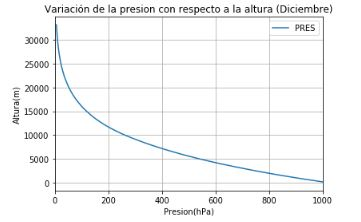
\includegraphics[width = \textwidth]{Presion_altura_dec.JPG}
%\caption{Variación de la presión respecto a la altura }

\end{subfigure}
\begin{subfigure}{0.49\textwidth}
\centering
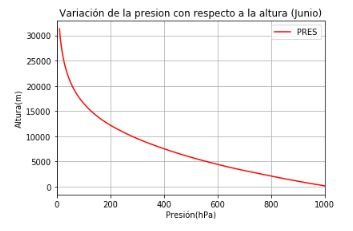
\includegraphics[width = \textwidth]{Presion_altura_jun.JPG}
%\caption{Right figure}

\end{subfigure}
\caption{Gráficas de presión como función de la altura}
\label{fig:combined}
\end{figure}

\newpage



Podemos ver en la \textbf{Figura 2} que en ambos meses la temperatura parece decrecer linealmente a partir de 12 km hacia abajo. En la gráfica de Diciembre, las temperaturas bajan hasta -70$^{\circ}$ a una altitud de 20-25 km, mientras que en la de Junio, las temperaturas bajan hasta -65$^{\circ}$ a una altitud de 15-20 km. 

\begin{figure}[ht!]
\centering
\begin{subfigure}{0.49\textwidth}
\centering
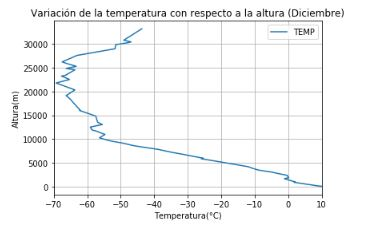
\includegraphics[width = \textwidth]{Temp_altura_dec.JPG}
%\caption{Variación de la presión respecto a la altura }

\end{subfigure}
\begin{subfigure}{0.49\textwidth}
\centering
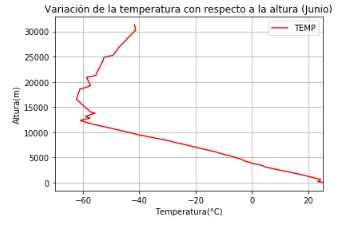
\includegraphics[width = \textwidth]{Temp_altura_jun.JPG}
%\caption{Right figure}

\end{subfigure}
\caption{Gráficas de temperatura como función de la altura}
\label{fig:combined}
\end{figure}

En la \textbf{Figura 3} podemos ver que la temperatura de rocío es más fría que la otra temperatura. En el mes de diciembre, ambas temperaturas van disminuyendo conforme la altitud incrementa en la troposfera hasta llegar a los 27.5 km (parte de la estratosfera) y empieza a incrementar la temperatura después de tal altitud.  
Podemos notar que en el intervalo de altura de 10 km en adelante, la diferencia entre las 2 temperaturas empieza a aumentar. En la gráfica de Junio se aprecia que la temperatura incrementa pasando los 15 km, en la estratosfera. 


\begin{figure}[ht!]
\centering
\begin{subfigure}{0.49\textwidth}
\centering
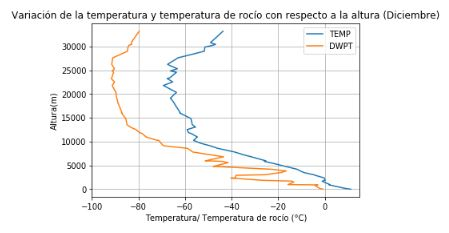
\includegraphics[width = \textwidth]{Temp_rocio_altura_dec.JPG}
%\caption{Variación de la presión respecto a la altura }

\end{subfigure}
\begin{subfigure}{0.49\textwidth}
\centering
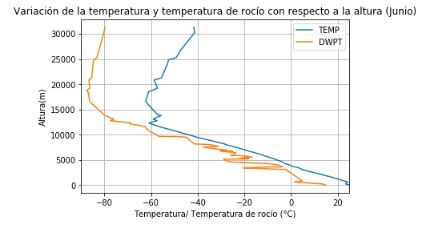
\includegraphics[width = \textwidth]{Temp_rocio_altura_jun.JPG}
%\caption{Right figure}

\end{subfigure}
\caption{Gráficas de temperatura y temperatura de rocío como función de la altura}
\label{fig:combined}
\end{figure}


En la \textbf{Figura 4} se hace notar que la humedad relativa es mayor en Junio que en Diciembre. Conforme aumenta la altitud, la humedad relativa tiende a disminuir para ambos casos. 


\begin{figure}[ht!]
\centering
\begin{subfigure}{0.49\textwidth}
\centering
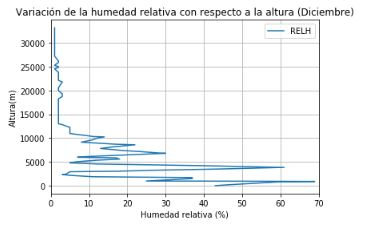
\includegraphics[width = \textwidth]{humedad_relativa_dec.JPG}
%\caption{Variación de la presión respecto a la altura }

\end{subfigure}
\begin{subfigure}{0.49\textwidth}
\centering
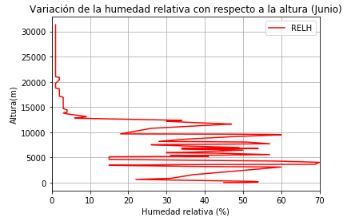
\includegraphics[width = \textwidth]{humedad_relativa_jun.JPG}
%\caption{Right figure}

\end{subfigure}
\caption{Gráficas de la humedad relativa como función de la altura}
\label{fig:combined}
\end{figure}

\newpage

En la \textbf{Figura 5} se puede notar que la rapidez de los vientos en Junio son más "caóticos" que en Diciembre. No obstante, las rapideces que están graficadas en Diciembre llegan hasta los 25 nudos a una altitud de 10 km y 30km, mientras que en la gráfica de Junio las velocidades llegan hasta alrededor de 180 nudos a una altura mayor de los 30 km. 
\begin{figure}[ht!]
\centering
\begin{subfigure}{0.49\textwidth}
\centering
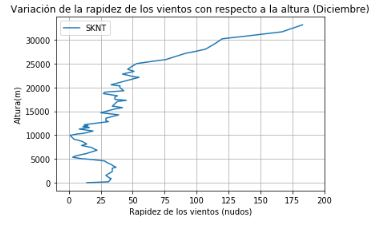
\includegraphics[width = \textwidth]{Rapidez_vientos_dec.JPG}
%\caption{Variación de la presión respecto a la altura }

\end{subfigure}
\begin{subfigure}{0.49\textwidth}
\centering
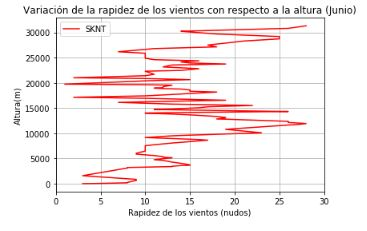
\includegraphics[width = \textwidth]{Rapidez_vientos_jun.JPG}
%\caption{Right figure}

\end{subfigure}
\caption{Gráficas de la rapidez de los vientos}
\label{fig:combined}
\end{figure}

\section{Conclusión}

Los globos meteorologicos son de gran utilidad a la hora de querer medir magnitudes meteorológicas a grandes altitudes. A partir de las gráficas obtenidas de los datos meteorológicos de Brindisi, Italia los días 22 de Diciembre 2017 y 22 de Junio 2017, se puede llegar a varias conclusiones. Primero, no se ve un cambio en la presión como función de la altura en esos dos días. Segundo, la temperatura parece decrecer linealmente por debajo de la estratosfera.Tercero, la humedad relativa de junio es mayor a diferentes altitudes en comparasión a la gráfica de diciembre. Finalmente, se presentan mayores rapideces de los vientos en el mes de Diciembre que en Junio. 

\section{Bibliografía}

\begin{itemize}
  \item Intro. to weather balloons, High Altitude Science. Recuperado el 12 de Febrero, 2018, de: \url{https://www.highaltitudescience.com/pages/intro-to-weather-balloons}
  \item Radiosonde, Wikipedia. Recuperado el 12 de Febrero, 2018, de: \url{https://en.wikipedia.org/wiki/Radiosonde}
  \item Punto de Rocío, Wikipedia. Recuperado el 12 de Febrero, 2018, de: \url{https://es.wikipedia.org/wiki/Punto_de_roc%C3%ADo}
  \item Radiosondes-An Upper Air Probe, Department of Atmospheric and Oceanic Sciences, University of Wisconsin-Madison. Recuperado el 12 de Febrero, 2018, de: \url{http://www.aos.wisc.edu/~hopkins/wx-inst/wxi-raob.htm}
  \item Upper air sounding, Department of Atmospheric Sciences, University of Wyoming. Recuperado el 8 de Febrero, 2018, de: \url{http://weather.uwyo.edu/upperair/sounding.html}
\end{itemize} 

\section{Apéndice}
{\parindent0pt
\textbf{1° ¿Cuál es tu opinión general de esta actividad?}

Considero que esta actividad nos acerca al análisis de datos reales y su interpretación. Esta actividad da seguimiento al tema que hemos estado viendo sobre la atmósfera de la tierra. 

\textbf{2° ¿Qué fue lo que más te agradó? ¿Lo que menos te agradó?}

Lo que más me agradó fue investigar acerca de los globos meteorológicos y su funcionamineto. No hubo nada que me desagradara. 

\textbf{3°¿Qué consideras que aprendiste en esta actividad?}

Sobre las magnitudes que pueden ser medidas por la radiosonda del globo meteorológico y ver gráficamente con datos reales, las relaciones entre ellas. 

\textbf{4° ¿Qué le faltó o le sobró?}

Estuvo muy completa la actividad, desde la captura de datos, la graficación de ellos, la investigación del marco teórico que ayuda a comprender los conceptos clave de la práctica y finalmente el análisis e interpretación de las gráficas. 

\textbf{5° ¿Qué mejoras sugieres a la actividad?}

Revisar de manera grupal los comandos esenciales para modificar las gráficas, así como su apariencia. 








\end{document}